\begin{figure}[H]
    \centering
    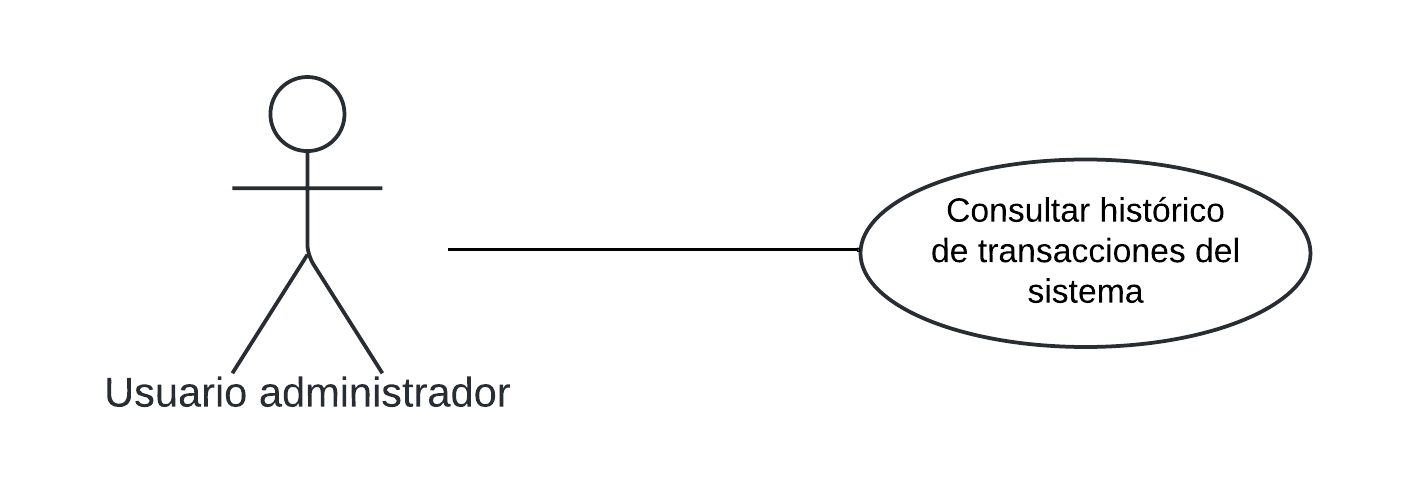
\includegraphics[width=0.5\textwidth]{figures/6-Analisis/6-Casos-uso/6_3_5_Gestion-transacciones.png}
    \caption{Casos de uso. Gestión de transacciones}
    \label{fig:cu_gestion-transacciones}
\end{figure}

\subsubsection{Caso de uso. Consultar histórico de transacciones del sistema} \label{sec:cu_transacciones-sistema}
\begin{longtable}{
   >{\columncolor{lightgreen!20}}p{4cm} % Primera columna con color de fondo verde claro
    >{\columncolor{white}}p{12cm}        % Segunda columna con color de fondo blanco (explícito)
    }
    \caption{Caso de uso. Histórico de transacciones del sistema} \label{table:cu_transacciones-sistema} \\
    \toprule
    \rowcolor{darkgreen!50} % Aplicando color de fondo verde oscuro a toda la fila
    \textbf{Caso de uso} & \centering\arraybackslash \textbf{HISTÓRICO DE TRANSACCIONES DEL SISTEMA} \\
    \endfirsthead
    
    \multicolumn{2}{c}%
    {\tablename\ \thetable{} -- continuación de la página anterior} \\
    \toprule
    \rowcolor{darkgreen!50}
    \textbf{Caso de uso} & \centering\arraybackslash \textbf{HISTÓRICO DE TRANSACCIONES DEL SISTEMA} \\
    \midrule
    \endhead
    
    \midrule
    \multicolumn{2}{r}{Continúa en la siguiente página...} \\ 
    \endfoot
    
    \bottomrule
    \endlastfoot
    
    \midrule
    Descripción & Un usuario administrador puede consultar el histórico de transacciones del sistema. \\
    \midrule
    Actores principales & Usuario administrador \\
    \midrule
    Actores secundarios &  \\
    \midrule
    Precondiciones & \begin{itemize}[nosep,leftmargin=*]
        \item El usuario ha iniciado sesión en el sistema.
    \end{itemize} \\
    \midrule
    Postcondiciones &  \\
    \midrule
    Disparadores & El usuario selecciona la opción de consultar el histórico de transacciones. \\
    \midrule
    Escenario principal & \begin{enumerate}[nosep,leftmargin=*]
        \item El sistema muestra el listado de transacciones realizadas en el sistema por los diferentes usuarios.
        \item El usuario puede filtrar las transacciones por diferentes criterios.
    \end{enumerate} \\
    \midrule
    Escenarios alternativos & 
    \begin{itemize}[nosep,leftmargin=*]
        \item \textbf{Escenario alternativo 1. No hay transacciones registradas.}
        \begin{enumerate}[nosep,leftmargin=*]
            \item El sistema muestra un mensaje indicando que no hay transacciones registradas.
        \end{enumerate}
    \end{itemize} \\
    \midrule
    Situaciones de error & 
    \begin{itemize}[nosep,leftmargin=*]
        \item \textbf{Error de conexión a la base de datos.}
        \begin{enumerate}[nosep,leftmargin=*]
            \item El sistema muestra un mensaje de error.
        \end{enumerate}
    \end{itemize} \\
\end{longtable}

